\chapter{Experimental setup}

\intro{The measurements within this thesis have been carried out by analyzing proton-proton collision data recorded with the CMS detector in 2012, 2015, and 2016 at center-of-mass energies of 8 and 13~\TeV. The experimental setup is described in this chapter. First, the \glsreset{lhc}\gls{lhc}, its preacceleator chain and other experiments at the \gls{lhc} are briefly introduced. Then the CMS detector and its components are detailed. A review of the operations summarizes the chapter.}

\section{Large Hadron Collider}

\subsection{Accelerator complex}

\myfigure{The accelerator complex at CERN. The figure is taken in parts from Ref.~\cite{Mobs:2225847}.}{
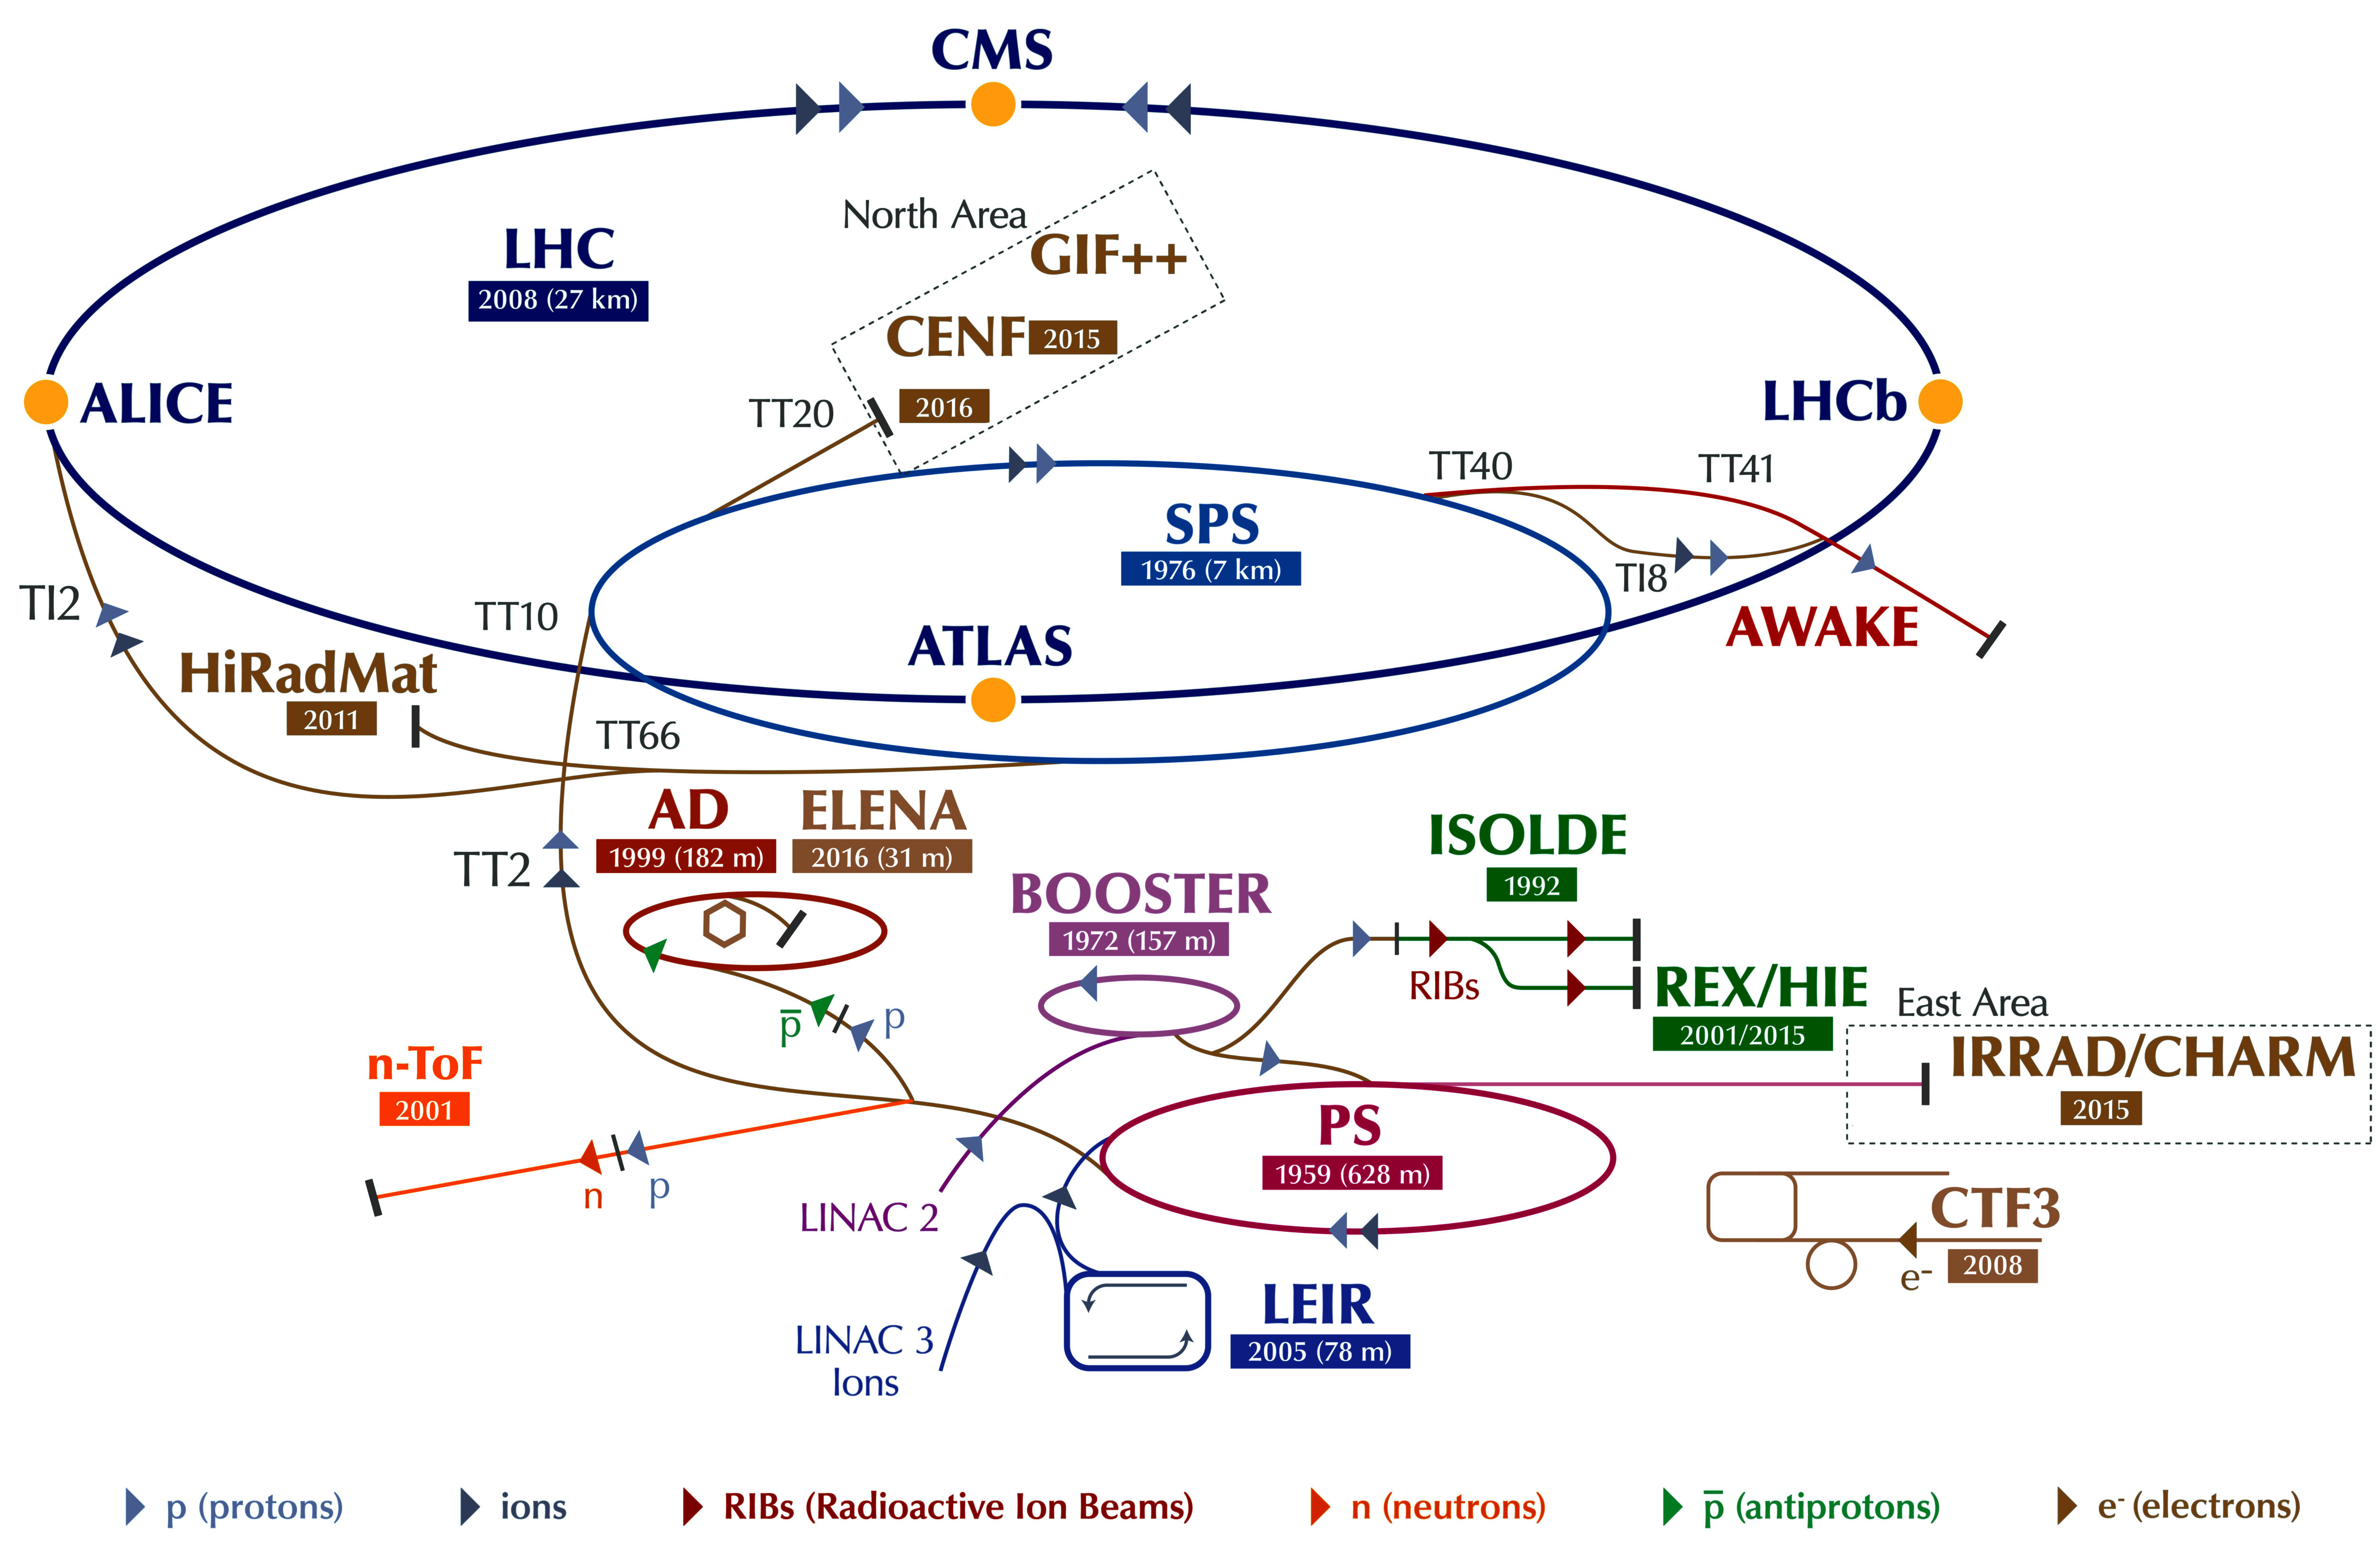
\includegraphics[width=0.99\textwidth]{figures/experiment/CERN_accelerator_complex.jpg}
}



momentum compaction

\subsection{Experiments}

\section{CMS experiment}

\subsection{Magnet}

\subsection{Tracker}

\cite{Chatrchyan:2014fea}

\subsection{Electromagnetic calorimeter}

\subsection{Hadronic calorimeter}

\subsection{Muon systems}
DT/RPC/CSC

\subsection{Data acquisition}
Trigger/DAQ

\subsection{Operations}
DCS/DSS
